% chapters/dpt.tex
% generated from dpt_energy_extraction.tex
\chapter{Extracting Eon, Eoff and Err from double pulse tests}
\label{ch:dpt}
\begin{chapabstract}
This note describes how to compute the switching energies $\Eon$, $\Eoff$ and $\Err$
from double pulse test (DPT) records consisting of the collector--emitter voltage
$\vce(t)$ and the emitter current $i_{\mathrm{E}}(t)$ sampled at
$T_s=\SI{2}{\nano\second}$. It covers the signal conditioning steps that dominate the
final uncertainty (offset removal, probe deskew, stray inductance), the integration
limits used by device manufacturers, the indirect determination of the diode
reverse-recovery energy when only the DUT is instrumented, and the numerical
implementation in MATLAB. The output is a set of energy values in the form required by
a lookup-table loss model.
\end{chapabstract}

\section{Test circuit and measured quantities}

The standard DPT circuit is shown in Fig.~\ref{dpt:fig:dpt}. The device under test (DUT) is
the low-side IGBT $T_2$; the load inductor $L_{\mathrm{load}}$ is connected between the
phase output and the positive rail, so that the load current freewheels through the
high-side diode $D_1$ when $T_2$ is off. The high-side IGBT $T_1$ is permanently off.

\begin{figure}[htbp]
\centering
\begin{circuitikz}[scale=1.0, transform shape, european]
  % DC link
  \draw (0,0) to[battery1, l=$\Vdc$] (0,4);
  \draw (0,4) -- (1.5,4);
  \draw (0,0) -- (1.5,0);
  \draw (1.5,4) to[C, l_=$C_{\mathrm{dc}}$] (1.5,0);
  \draw (1.5,4) -- (4.2,4);
  \draw (1.5,0) -- (4.2,0);

  % high-side IGBT and diode
  \node[nigbt] (T1) at (4.2,2.8) {};
  \draw (T1.C) -- (4.2,4);
  \draw (T1.E) -- (4.2,1.6);
  \draw (T1.G) -- ++(-0.5,0) node[left]{\footnotesize off};
  \draw (5.4,2.1) to[D*, l_=$D_1$] (5.4,3.5);
  \draw (4.2,3.5) -- (5.4,3.5);
  \draw (4.2,2.1) -- (5.4,2.1);

  % load inductor
  \draw (4.2,4) -- (7.8,4);
  \draw (7.8,4) to[L, l=$L_{\mathrm{load}}$] (7.8,1.6);
  \draw (7.8,1.6) -- (4.2,1.6);

  % low-side DUT and diode
  \node[nigbt] (T2) at (4.2,1.05) {};
  \draw (T2.C) -- (4.2,1.6);
  \draw (T2.E) -- (4.2,0);
  \draw (T2.G) to[R, l_=$R_{\mathrm{G}}$] (2.0,1.05) node[left]{\footnotesize driver};
  \draw (5.4,0.15) to[D*, l_=$D_2$] (5.4,1.55);
  \draw (4.2,1.55) -- (5.4,1.55);
  \draw (4.2,0.15) -- (5.4,0.15);

  % probes
  \draw[<->, red, thick] (6.5,1.55) -- (6.5,0.15);
  \node[red, right] at (6.5,0.85) {$\vce(t)$};
  \draw[red, thick] (4.2,0.5) circle (0.22);
  \node[red, left] at (3.9,0.42) {$i_{\mathrm{E}}(t)$};
\end{circuitikz}
\caption{Double pulse test circuit. DUT: low-side IGBT $T_2$; commutation partner:
high-side diode $D_1$.}
\label{dpt:fig:dpt}
\end{figure}

The gate command consists of two pulses. The first, long pulse magnetises
$L_{\mathrm{load}}$ up to the target current; the short off-interval between the two
pulses produces the turn-off event; the second pulse produces the turn-on event. Only the
\emph{first turn-off} and the \emph{second turn-on} are evaluated, because only for these
two transitions is the current well defined and the device in a thermally and
electrically settled state.

The two recorded channels are
\begin{align}
\vce(t) &\quad \text{measured at the module power terminals (C and E),}\\
i_{\mathrm{E}}(t) &\quad \text{measured in the emitter lead.}
\end{align}
Since the gate current is at most a few amperes and flows only for tens of nanoseconds,
$i_{\mathrm{E}}(t)\simeq\ic(t)$ is assumed throughout; if a coaxial shunt in the emitter
lead is used, the gate-current contribution can be subtracted if $i_{\mathrm{G}}$ is
recorded.

\section{Signal conditioning}

The numerical integration itself is trivial. Essentially all the achievable accuracy is
decided in the pre-processing.

\subsection{Offset and baseline removal}

Both channels must have zero mean over an interval in which the physical quantity is
known to be zero:
\begin{equation}
\hat{\imath}(t) = i(t) - \frac{1}{N_0}\sum_{k\in\mathcal{W}_0} i(t_k),
\end{equation}
where $\mathcal{W}_0$ is a pre-trigger window (typically \SIrange{1}{5}{\micro\second})
taken before the first gate pulse, where the current is exactly zero. The same applies to
$\vce$ only if a window exists where the device is fully on; otherwise the voltage offset
is calibrated separately.

With $\IL=\SI{1200}{\ampere}$ and a typical overlap duration of \SI{300}{\nano\second}, a
current offset of \SI{5}{\ampere} already produces an error of the order of
\SI{1.4}{\milli\joule} on $\Eon$. Rogowski coils additionally suffer from integrator
droop: the baseline must be estimated \emph{immediately} before the transient, not at the
beginning of the record.

\subsection{Probe deskew}

This is the dominant error source. Let $\delta$ be the residual time misalignment between
the current and the voltage channel. The measured energy is
\begin{equation}
E(\delta)=\int v(t)\, i(t+\delta)\,\mathrm{d}t
\simeq E(0)+\delta\int v(t)\,\frac{\mathrm{d}i}{\mathrm{d}t}\,\mathrm{d}t .
\end{equation}
During turn-off the voltage is close to $\Vdc$ while the current falls from $\IL$ to
zero, hence $\int v\,\mathrm{d}i \simeq -\Vdc \IL$ and
\begin{equation}
\boxed{\;\left|\frac{\Delta E}{E}\right| \simeq \frac{\Vdc\,\IL}{E}\,|\delta|
= \frac{|\delta|}{\tau_{\mathrm{eq}}},\qquad
\tau_{\mathrm{eq}}\triangleq\frac{E}{\Vdc \IL}\;}
\label{dpt:eq:deskew}
\end{equation}
where $\tau_{\mathrm{eq}}$ is the equivalent rectangular overlap time. For
$\Vdc=\SI{900}{\volt}$, $\IL=\SI{1200}{\ampere}$ and $E\approx\SI{300}{\milli\joule}$ one
gets $\tau_{\mathrm{eq}}\approx\SI{278}{\nano\second}$: a deskew error of
\SI{10}{\nano\second} (five samples at $T_s=\SI{2}{\nano\second}$) causes a
\SI{3.6}{\percent} energy error, and the errors on $\Eon$ and $\Eoff$ have
\emph{opposite} sign, so the sum is much less sensitive than the individual terms.

Two practical procedures:
\begin{enumerate}
\item \textbf{Hardware}: use a deskew fixture before the measurement campaign. This is the
only reliable method and should always be preferred.
\item \textbf{Software}: exploit the fact that the instantaneous power dissipated in a
passive device cannot be significantly negative. Define
\begin{equation}
J(\delta)=\int_{t_1}^{t_2}\big[\max\!\big(0,\,-v(t)\,i(t+\delta)\big)\big]^2\mathrm{d}t,
\qquad \delta^\star=\arg\min_\delta J(\delta),
\label{dpt:eq:softdeskew}
\end{equation}
evaluated on the turn-on transient, where a skew produces a large spurious negative
power lobe. Sub-sample resolution is obtained by interpolating $i$ on a shifted grid.
This is a correction, not a substitute for hardware deskew.
\end{enumerate}

\subsection{Bandwidth and sampling}

At $T_s=\SI{2}{\nano\second}$ the Nyquist frequency is \SI{250}{\mega\hertz}, adequate for
a \SI{1700}{\volt} Si IGBT whose transients contain little energy above
\SI{100}{\mega\hertz}. With $\mathrm{d}v/\mathrm{d}t=\SI{5}{\kilo\volt\per\micro\second}$
the voltage moves \SI{10}{\volt} per sample and with
$\mathrm{d}i/\mathrm{d}t=\SI{5}{\kilo\ampere\per\micro\second}$ the current moves
\SI{10}{\ampere} per sample: the trapezoidal rule then has a truncation error well below
\SI{0.1}{\percent}. A convergence check is obtained by decimating the record by factors
2, 4, 8 and verifying that the energy changes by less than the target tolerance.

\subsection{Stray inductance}

The voltage measured at the power terminals contains the drop across the internal
inductance $L_\sigma$ between the sensing points and the chip:
\begin{equation}
\vce^{\mathrm{term}}(t)=v_{\mathrm{chip}}(t)+L_\sigma\frac{\mathrm{d}\ic}{\mathrm{d}t}.
\end{equation}
Integrating the difference gives a closed-form bias:
\begin{equation}
E^{\mathrm{term}}-E^{\mathrm{chip}}
=\int L_\sigma \frac{\mathrm{d}\ic}{\mathrm{d}t}\,\ic \,\mathrm{d}t
=\tfrac{1}{2}L_\sigma\left(I_{\mathrm{end}}^2-I_{\mathrm{start}}^2\right),
\label{dpt:eq:Lsigma}
\end{equation}
i.e.\ $+\tfrac{1}{2}L_\sigma \IL^2$ at turn-on and $-\tfrac{1}{2}L_\sigma \IL^2$ at
turn-off. With $L_\sigma=\SI{15}{\nano\henry}$ and $\IL=\SI{1200}{\ampere}$ this is
\SI{10.8}{\milli\joule} per transition.

Two remarks:
\begin{itemize}
\item Manufacturers integrate the \emph{terminal} quantities. If the objective is to
reproduce or verify datasheet numbers, no de-embedding must be applied.
\item The \emph{external} commutation-loop inductance shifts energy between $\Eon$ and
$\Eoff$ (the rail collapse during turn-on lowers the measured $\Eon$, the overvoltage at
turn-off raises the measured $\Eoff$). The sum $\Eon+\Eoff+\Err$ is therefore far more
representative of the test bench than each individual term, and any comparison against
datasheet values must be made at comparable loop inductance.
\end{itemize}

\section{Definitions}

The instantaneous dissipated power of the DUT is
\begin{equation}
p(t)=\vce(t)\,\ic(t),
\end{equation}
and the switching energy is its integral over an interval whose limits are conventional:
\begin{equation}
E=\int_{t_1}^{t_2}\vce(t)\,\ic(t)\,\mathrm{d}t .
\end{equation}

\subsection{Operating point}

Both integration limits and the reported operating point are referred to the two levels
\begin{equation}
\Vdc = \left\langle \vce(t)\right\rangle_{t\in\mathcal{W}_{\mathrm{off}}},
\qquad
\IL = \left\langle \ic(t)\right\rangle_{t\in\mathcal{W}_{\mathrm{on}}},
\end{equation}
where $\mathcal{W}_{\mathrm{off}}$ is a window in the off-state well after the ringing has
decayed (a few \si{\micro\second} before the second turn-on) and
$\mathcal{W}_{\mathrm{on}}$ is a window of \SIrange{0.2}{1}{\micro\second} immediately
before the turn-off command. Note that, because of the inductor magnetisation during the
off-time and the DC-link droop, the current at turn-off and at turn-on differ slightly:
each energy must be reported with \emph{its own} current.

\subsection{Integration limits}

The conventional limits, consistent with IEC 60747-9 and with the definitions used in
IGBT module datasheets, are summarised in Table~\ref{dpt:tab:limits} and illustrated in
Fig.~\ref{dpt:fig:limits}.

\begin{table}[htbp]
\centering
\caption{Integration limits.}
\label{dpt:tab:limits}
\begin{tabular}{llll}
\toprule
Energy & Start $t_1$ & Stop $t_2$ & Integrand \\
\midrule
$\Eon$  & $\ic \uparrow 0.10\,\IL$ & $\vce \downarrow 0.02\,\Vdc$ & $\vce \ic$ \\
$\Eoff$ & $\vce \uparrow 0.10\,\Vdc$ & $\ic \downarrow 0.02\,\IL$ & $\vce \ic$ \\
$\Err$  & $i_{\mathrm{D}} \downarrow 0$ & $|i_{\mathrm{D}}| \downarrow 0.02\,I_{\mathrm{rrm}}$ & $v_{\mathrm{D}} i_{\mathrm{D}}$ \\
\bottomrule
\end{tabular}
\end{table}

Formally, with $\alpha=0.10$ and $\beta=0.02$,
\begin{align}
t_{1}^{\mathrm{on}}  &= \min\{t: \ic(t)\ge \alpha \IL\}, &
t_{2}^{\mathrm{on}}  &= \min\{t>t_1^{\mathrm{on}}: \vce(t)\le \beta \Vdc\}, \\
t_{1}^{\mathrm{off}} &= \min\{t: \vce(t)\ge \alpha \Vdc\}, &
t_{2}^{\mathrm{off}} &= \min\{t>t_1^{\mathrm{off}}: \ic(t)\le \beta \IL\}.
\end{align}
The crossing instants must be found by linear interpolation between samples, not by
sample indexing, and the signals must be lightly filtered (or the crossing detected with
hysteresis) so that ringing does not trigger a false crossing.

\begin{figure}[htbp]
\centering
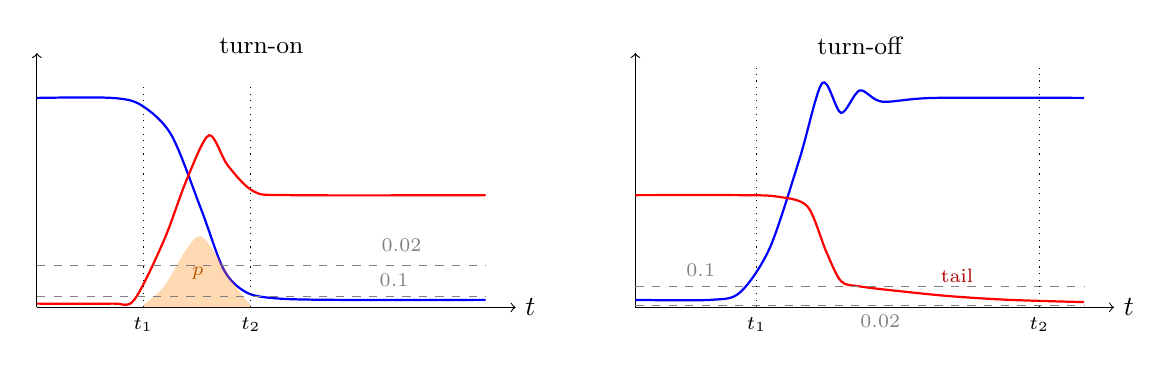
\begin{tikzpicture}[scale=0.95]
% ---------------- turn-on -----------------
\begin{scope}
  \draw[->] (0,0) -- (6.4,0) node[right]{$t$};
  \draw[->] (0,0) -- (0,3.4) node[above]{};
  \node at (3,3.5) {\small turn-on};
  % vce
  \draw[thick, blue] plot[smooth] coordinates
    {(0,2.8)(1.0,2.8)(1.4,2.7)(1.8,2.3)(2.2,1.3)(2.5,0.5)(2.8,0.2)(3.2,0.12)(4.0,0.1)(6.0,0.1)};
  \node[blue, above right] at (0.1,2.8) {$\vce$};
  % ic
  \draw[thick, red] plot[smooth] coordinates
    {(0,0.05)(1.0,0.05)(1.3,0.1)(1.7,0.9)(2.0,1.7)(2.3,2.3)(2.55,1.9)(2.9,1.55)(3.4,1.5)(6.0,1.5)};
  \node[red, above right] at (4.2,1.5) {$\ic$};
  % thresholds
  \fill[orange, opacity=0.30] (1.42,0) -- plot[smooth] coordinates
    {(1.42,0.03)(1.7,0.28)(2.0,0.78)(2.2,0.95)(2.45,0.62)(2.7,0.22)(2.86,0.03)} -- (2.86,0) -- cycle;
  \node[orange!70!black] at (2.15,0.45) {\scriptsize $p$};
  \draw[dashed, gray] (0,0.15) -- (6.0,0.15);
  \node[gray, above, font=\scriptsize] at (4.8,0.15) {$0.1\,\IL$};
  \draw[dotted] (1.42,0) -- (1.42,3.0);
  \draw[dotted] (2.86,0) -- (2.86,3.0);
  \node[below] at (1.42,0) {\scriptsize $t_1$};
  \node[below] at (2.86,0) {\scriptsize $t_2$};
  \node[gray, above, font=\scriptsize] at (4.9,0.62) {$0.02\,\Vdc$};
  \draw[dashed, gray] (0,0.56) -- (6.0,0.56);
\end{scope}
% ---------------- turn-off -----------------
\begin{scope}[xshift=8cm]
  \draw[->] (0,0) -- (6.4,0) node[right]{$t$};
  \draw[->] (0,0) -- (0,3.4);
  \node at (3,3.5) {\small turn-off};
  % vce
  \draw[thick, blue] plot[smooth] coordinates
    {(0,0.1)(1.0,0.1)(1.4,0.2)(1.8,0.8)(2.2,2.0)(2.5,3.0)(2.75,2.6)(3.0,2.9)(3.3,2.75)(4.0,2.8)(6.0,2.8)};
  \node[blue, above right] at (4.2,2.8) {$\vce$};
  % ic with tail
  \draw[thick, red] plot[smooth] coordinates
    {(0,1.5)(1.4,1.5)(1.9,1.48)(2.3,1.35)(2.55,0.75)(2.75,0.35)(3.0,0.28)(3.5,0.22)(4.2,0.15)(5.0,0.1)(6.0,0.07)};
  \node[red, above right] at (0.1,1.55) {$\ic$};
  \node[red!70!black] at (4.3,0.42) {\scriptsize tail};
  % thresholds
  \draw[dashed, gray] (0,0.28) -- (6.0,0.28);
  \node[gray, above, font=\scriptsize] at (0.9,0.28) {$0.1\,\Vdc$};
  \draw[dashed, gray] (0,0.03) -- (6.0,0.03);
  \node[gray, below, font=\scriptsize] at (3.3,0.03) {$0.02\,\IL$};
  \draw[dotted] (1.62,0) -- (1.62,3.2);
  \draw[dotted] (5.4,0) -- (5.4,3.2);
  \node[below] at (1.62,0) {\scriptsize $t_1$};
  \node[below] at (5.4,0) {\scriptsize $t_2$};
\end{scope}
\end{tikzpicture}
\caption{Integration limits for turn-on (left) and turn-off (right). The turn-on current
peak is the reverse recovery of the opposite diode; the turn-off current tail is the
recombination of the drift-region excess carriers.}
\label{dpt:fig:limits}
\end{figure}

\subsection{The turn-off tail}

For an IGBT the $\beta=0.02$ criterion applied to the current is critical. At
$\IL=\SI{1200}{\ampere}$ the stop threshold is \SI{24}{\ampere}, and the tail current may
still exceed this level for several microseconds while the full DC-link voltage is
applied: a \SI{20}{\ampere} tail at \SI{900}{\volt} for \SI{2}{\micro\second} carries
\SI{36}{\milli\joule}, i.e.\ around \SI{10}{\percent} of $\Eoff$. Two rules follow:
\begin{itemize}
\item the acquisition window after turn-off must be long enough
(\SIrange{10}{20}{\micro\second}), otherwise the tail is truncated by the record, not by
the criterion;
\item the current channel must be accurate at the ampere level while ranged for
\SI{1200}{\ampere}. This is the practical reason why the tail contribution is the least
reproducible part of $\Eoff$.
\end{itemize}
It is good practice to report $\Eoff$ together with its sensitivity, e.g.\ the value
obtained with $\beta=0.02$ and with a fixed \SI{10}{\micro\second} window.

\section{Reverse recovery energy from the DUT waveforms}

$\Err$ belongs to the diode $D_1$, which is normally not instrumented. It can be
reconstructed from the DUT channels because the commutation loop imposes two algebraic
relations. Taking the diode current $i_{\mathrm{D}}$ positive in the forward direction and
the diode voltage $v_{\mathrm{D}}$ as anode-to-cathode:
\begin{align}
i_{\mathrm{D}}(t) &= \IL - \ic(t), \label{dpt:eq:iD}\\
v_{\mathrm{D}}(t) &= \vce(t) - \Vdc + L_{\sigma,\mathrm{dc}}\frac{\mathrm{d}\ic}{\mathrm{d}t}
\;\simeq\; \vce(t)-\Vdc . \label{dpt:eq:vD}
\end{align}
Therefore
\begin{equation}
\boxed{\;
\Err = \int_{t_1^{\mathrm{rr}}}^{t_2^{\mathrm{rr}}}
\big(\Vdc-\vce(t)\big)\,\big(\ic(t)-\IL\big)\,\mathrm{d}t \;}
\label{dpt:eq:Err}
\end{equation}
which is non-negative during recovery, since there $\ic>\IL$ and $\vce<\Vdc$. The limits
are
\begin{align}
t_1^{\mathrm{rr}} &= \min\{t:\ \ic(t)\ge \IL\} \quad(\text{diode current zero crossing}),\\
t_2^{\mathrm{rr}} &= \min\{t>t_{\mathrm{peak}}:\ \ic(t)-\IL \le 0.02\,I_{\mathrm{rrm}}\},
\qquad I_{\mathrm{rrm}}=\max_t\big(\ic(t)-\IL\big).
\end{align}
The recovery charge, useful as a cross-check and for parameterising a diode model, is
\begin{equation}
Q_{\mathrm{rr}}=\int_{t_1^{\mathrm{rr}}}^{t_2^{\mathrm{rr}}}\big(\ic(t)-\IL\big)\,\mathrm{d}t,
\qquad \text{with the consistency check } \Err \approx k\,Q_{\mathrm{rr}}\Vdc,\ k\in[0.4,0.6].
\end{equation}

Limitations of the indirect method, to be stated explicitly whenever it is used:
\begin{itemize}
\item $\Vdc$ is assumed constant, whereas the rail collapses by
$L_{\sigma,\mathrm{dc}}\,\mathrm{d}i/\mathrm{d}t$ during the current rise. If a probe is
available on the DC-link close to the module, $\Vdc$ should be replaced by the measured
instantaneous rail voltage, and \eqref{dpt:eq:vD} becomes exact up to the residual layout
inductance.
\item The inductance between the two chips is attributed entirely to one device, so the
split between $\Eon$ and $\Err$ is affected while $\Eon+\Err$ is not.
\item The diode forward conduction before the zero crossing is excluded by construction,
which is consistent with the datasheet definition of $\Err$.
\end{itemize}
Note also that $\Eon$ of the IGBT computed as in Table~\ref{dpt:tab:limits} \emph{already
includes} the effect of the recovery current, because the recovery peak flows through the
IGBT: $\Eon$ and $\Err$ must not be corrected for double counting, they are two distinct
energies dissipated in two distinct chips.

\section{Numerical implementation}

\subsection{Crossing detection}

Given a signal $x$ sampled on a uniform grid and a threshold $X$, the crossing instant is
obtained by linear interpolation between the two samples that bracket it:
\begin{equation}
t^\star = t_k + T_s\,\frac{X-x_k}{x_{k+1}-x_k},\qquad
k=\min\{j:\ (x_j-X)(x_{j+1}-X)\le 0\}.
\end{equation}
The integral over $[t_1,t_2]$ with non-grid endpoints is computed with the trapezoidal
rule on the interior samples plus the two partial trapezoids at the ends; the values
$p(t_1)$ and $p(t_2)$ are themselves obtained by linear interpolation.

\subsection{MATLAB code}

\begin{lstlisting}[caption={Utility functions: threshold crossing and interpolated integral.}]
function tc = tcross(t, x, level, dir, tstart)
% First instant after TSTART at which X crosses LEVEL in direction DIR (+1/-1).
    if nargin < 5, tstart = t(1); end
    i0 = find(t >= tstart, 1, 'first');
    s  = dir*(x(i0:end) - level);
    k  = find(s(1:end-1) < 0 & s(2:end) >= 0, 1, 'first');
    if isempty(k), tc = NaN; return; end
    k  = k + i0 - 1;
    tc = t(k) + (t(k+1)-t(k))*(level-x(k))/(x(k+1)-x(k));
end

function E = trapz_interval(t, p, t1, t2)
% Trapezoidal integral of P(t) between arbitrary instants T1 and T2.
    m  = t > t1 & t < t2;
    p1 = interp1(t, p, t1);   p2 = interp1(t, p, t2);
    tt = [t1;  t(m);  t2];
    pp = [p1;  p(m);  p2];
    E  = trapz(tt, pp);
end
\end{lstlisting}

\begin{lstlisting}[caption={Pre-processing: offset removal and deskew.}]
function [t, v, i] = dpt_prepare(t, v, i, w0, delta)
% W0    : [t_start t_stop] pre-trigger window with i == 0
% DELTA : current-channel delay to be compensated [s] (i is shifted by -DELTA)
    t = t(:); v = v(:); i = i(:);
    m = t >= w0(1) & t <= w0(2);
    i = i - mean(i(m));                       % current offset
    if nargin >= 5 && delta ~= 0
        i = interp1(t, i, t + delta, 'pchip', 'extrap');
    end
end
\end{lstlisting}

\begin{lstlisting}[caption={Operating point and switching energies.}]
function S = dpt_energies(t, v, i, tOff, tOn, opt)
% TOFF, TON : approximate instants of the turn-off and turn-on commands [s]
% OPT.alpha (0.10), OPT.beta (0.02), OPT.wOn, OPT.wOff : averaging windows [s]

    if ~isfield(opt,'alpha'), opt.alpha = 0.10; end
    if ~isfield(opt,'beta'),  opt.beta  = 0.02; end
    if ~isfield(opt,'wOn'),   opt.wOn   = 0.5e-6; end   % before turn-off
    if ~isfield(opt,'wOff'),  opt.wOff  = 2.0e-6; end   % before turn-on

    % ---- operating point -------------------------------------------------
    mI  = t > tOff - opt.wOn  & t < tOff - 50e-9;
    mV  = t > tOn  - opt.wOff & t < tOn  - 50e-9;
    IL  = mean(i(mI));            % load current at turn-off
    Vdc = mean(v(mV));            % blocking voltage before turn-on

    p = v.*i;                     % instantaneous power [W]

    % ---- turn-off --------------------------------------------------------
    t1 = tcross(t, v, opt.alpha*Vdc, +1, tOff - 100e-9);
    t2 = tcross(t, i, opt.beta *IL,  -1, t1);
    S.Eoff  = trapz_interval(t, p, t1, t2);
    S.toff  = [t1 t2];

    % ---- turn-on ---------------------------------------------------------
    ILon = mean(i(t > tOn + 3e-6 & t < tOn + 4e-6));   % current after turn-on
    t3 = tcross(t, i, opt.alpha*ILon, +1, tOn - 100e-9);
    t4 = tcross(t, v, opt.beta *Vdc,  -1, t3);
    S.Eon = trapz_interval(t, p, t3, t4);
    S.ton = [t3 t4];

    % ---- reverse recovery of the opposite diode --------------------------
    irr  = i - ILon;                       % diode current = ILon - i
    vrr  = Vdc - v;                        % diode reverse voltage
    t5   = tcross(t, i, ILon, +1, t3);     % diode current zero crossing
    mpk  = t > t5 & t < t5 + 2e-6;
    [Irrm, kpk] = max(irr(mpk));
    idx  = find(mpk, 1, 'first') + kpk - 1;
    t6   = tcross(t, irr, opt.beta*Irrm, -1, t(idx));
    S.Err  = trapz_interval(t, vrr.*irr, t5, t6);
    S.Qrr  = trapz_interval(t, irr,      t5, t6);
    S.Irrm = Irrm;
    S.trr  = [t5 t6];

    % ---- operating point and checks --------------------------------------
    S.IL   = IL;  S.ILon = ILon;  S.Vdc = Vdc;
    S.Etot = S.Eon + S.Eoff + S.Err;
    S.k    = S.Err/(S.Qrr*Vdc);            % expected 0.4 ... 0.6
end
\end{lstlisting}

\begin{lstlisting}[caption={Software deskew estimate based on the non-negative power criterion.}]
function d = dpt_deskew(t, v, i, tOn, span)
% Minimises the spurious negative-power lobe on the turn-on transient.
    if nargin < 5, span = 1e-6; end
    m  = t > tOn - 0.2e-6 & t < tOn + span;
    dd = (-20:0.25:20)*1e-9;               % +/- 20 ns, 0.25 ns resolution
    J  = zeros(size(dd));
    for k = 1:numel(dd)
        is  = interp1(t, i, t + dd(k), 'pchip', 'extrap');
        p   = v(m).*is(m);
        J(k) = trapz(t(m), max(0,-p).^2);
    end
    [~,k0] = min(J);  d = dd(k0);
end
\end{lstlisting}

\subsection{Convergence and sensitivity checks}

Every extracted value should be accompanied by the following checks:
\begin{enumerate}
\item \textbf{Decimation}: recompute with $T_s$, $2T_s$, $4T_s$; the variation must be
below \SI{0.5}{\percent}.
\item \textbf{Threshold sensitivity}: recompute with $(\alpha,\beta)=(0.10,0.02)$,
$(0.05,0.01)$ and $(0.10,0.05)$; the spread is a realistic estimate of the definition
uncertainty and is typically a few percent for $\Eon$ and up to \SI{10}{\percent} for
$\Eoff$ because of the tail.
\item \textbf{Deskew sensitivity}: recompute with $\delta \pm \SI{2}{\nano\second}$ and
apply \eqref{dpt:eq:deskew}.
\item \textbf{Charge balance}: $Q_{\mathrm{rr}}$ from the current integral must be
consistent with the datasheet at the same $\mathrm{d}i/\mathrm{d}t$ and $T_{\mathrm{vj}}$.
\item \textbf{Energy balance}: $\Eon+\Eoff+\Err$ is the quantity that should be compared
across benches; individual terms depend on the loop inductance.
\end{enumerate}

\section{From single events to a loss model}

A DPT campaign sweeps the current and, if the bench allows it, the voltage, the gate
resistance and the junction temperature. The resulting data set is condensed as follows.

\subsection{Current dependence}

For a given $(\Vdc, R_{\mathrm{G}}, T_{\mathrm{vj}})$ the energies are well represented by
a second-order polynomial through the measured points:
\begin{equation}
E(I) = a_0 + a_1 I + a_2 I^2 .
\end{equation}
$a_0$ absorbs the voltage-dependent, current-independent part (displacement currents,
recovery of the residual charge); imposing $a_0=0$ is not recommended because it biases
the fit at high current, which is where the loss actually matters.

\subsection{Voltage dependence}

Over a limited range around the reference voltage a power law is adequate:
\begin{equation}
E(\Vdc)=E_{\mathrm{ref}}\left(\frac{\Vdc}{V_{\mathrm{ref}}}\right)^{K_v},
\end{equation}
with $K_v$ identified from at least three voltage levels. Typical values for Si IGBT
modules are $K_v\approx1.2\ldots1.4$ for $\Eon$ and $\Err$ and $K_v\approx1.0\ldots1.2$
for $\Eoff$; a linear scaling ($K_v=1$) is the usual first approximation and
underestimates $\Eon$ at high voltage.

\subsection{Temperature dependence}

Linear interpolation between two characterised temperatures is standard:
\begin{equation}
E(T_{\mathrm{vj}})=E_{25}+\big(E_{150}-E_{25}\big)\frac{T_{\mathrm{vj}}-25}{125}.
\end{equation}
The temperature coefficient is small for $\Eon$, moderate for $\Eoff$ (longer tail) and
large for $\Err$ (higher carrier lifetime and stored charge).

\subsection{Table for a lookup-table loss model}

The final deliverable is a table in the form of Table~\ref{dpt:tab:out}, one block per
$(\Vdc, R_{\mathrm{G}}, T_{\mathrm{vj}})$ combination, directly usable as breakpoints in
a Simscape or Simulink loss model. Reported currents must be the measured $\IL$ values,
not the nominal set points.

\begin{table}[htbp]
\centering
\caption{Output format of the extraction (values to be filled with the measured data).}
\label{dpt:tab:out}
\begin{tabular}{ccccccc}
\toprule
$\IL$ (\si{\ampere}) & $\Vdc$ (\si{\volt}) & $T_{\mathrm{vj}}$ (\si{\celsius}) &
$\Eon$ (\si{\milli\joule}) & $\Eoff$ (\si{\milli\joule}) &
$\Err$ (\si{\milli\joule}) & $Q_{\mathrm{rr}}$ (\si{\micro\coulomb}) \\
\midrule
300  & 900 & 150 & & & & \\
600  & 900 & 150 & & & & \\
900  & 900 & 150 & & & & \\
1200 & 900 & 150 & & & & \\
1800 & 900 & 150 & & & & \\
\bottomrule
\end{tabular}
\end{table}

\section{Checklist}

\begin{enumerate}
\item Verify the record contains a sufficient pre-trigger interval and at least
\SI{10}{\micro\second} after turn-off.
\item Remove the current offset on the window immediately preceding the transient.
\item Apply the hardware deskew; verify with \eqref{dpt:eq:softdeskew}.
\item Extract $\Vdc$ and $\IL$ (separately for the turn-off and turn-on events).
\item Locate $t_1,t_2$ by interpolated threshold crossing with $\alpha=0.10$,
$\beta=0.02$.
\item Integrate $p=\vce\ic$ for $\Eon$ and $\Eoff$; integrate
$(\Vdc-\vce)(\ic-\IL)$ for $\Err$.
\item Run the convergence and sensitivity checks; report the spread together with the
value.
\item Compare $\Eon+\Eoff+\Err$, not the individual terms, when validating against the
datasheet, and only at comparable $R_{\mathrm{G}}$, $L_\sigma$ and $T_{\mathrm{vj}}$.
\end{enumerate}

For \SI{1700}{\volt} modules the reference DC-link voltage used by manufacturers for the
datasheet switching energies is \SI{900}{\volt}, and $\Eon$ and $\Err$ refer to the
commutation between the DUT and the diode of the opposite switch, so that the two
energies share the same $\mathrm{d}i/\mathrm{d}t$ only if the gate resistances are the
ones specified in the datasheet.

